\section{Concepts as directions}
\label{sec:directions}

\begin{sessioncard}
\textbf{Session 3.} \emph{Goal:} understand the main working hypothesis of mechanistic interpretability, namely
that a model represents a concept as a direction in the space of its activations. We also learn the two basic
tools that come with this hypothesis: the probe, which looks for such a direction, and steering, which tests
whether the model uses the direction.
\emph{Experiments:} a probe for the gender of a name (\cref{exp:probe}), steering along the direction that the
probe suggests (\cref{exp:steer}), and a result that shows why finding a direction and testing it are two
different things (\cref{exp:decodable}).
\emph{Prerequisites:} sessions 1 and 2.
\end{sessioncard}

\subsection{From components to concepts}

Session 2 described the model in terms of the parts of its architecture: layers, heads and positions. To
describe what a model represents, we need a second kind of unit, which corresponds to a concept. We use the word
\emph{feature} for a property of the input, or of the model's intermediate computation, that the model represents
internally because the property helps to predict the next token. Examples are ``the current token is a first
name'', ``this text is French'' or ``this name has occurred before''. This definition is deliberately informal,
because nobody knows yet how to make it precise.

The simplest possible design would give each feature its own coordinate of the stream. But we saw in
\cref{sec:facts} that the coordinates of the stream play no special role, so there is no reason to expect this
design. The next simplest possibility is that each feature corresponds to a \emph{direction} in the stream.

\begin{definition}[Linear representation hypothesis, working form]\label{def:lrh}
For an activation $x\in\R^d$ at a fixed place in the model (for example, the stream at the input of a given layer) there
are unit vectors $v_1,\dots,v_N\in\R^d$, called \emph{feature directions}, and non-negative functions
$f_1,\dots,f_N$ of the input, called \emph{feature activations}, such that
\begin{equation}\label{eq:lrh}
x \;\approx\; \sum_{j=1}^{N}f_j\,v_j
\end{equation}
on all inputs of interest, where each $f_j$ measures the presence of one feature and only few of the $f_j$ are
nonzero on any single input.
\end{definition}

In words, each feature corresponds to a direction, and the strength of the feature is the length of $x$ along
this direction. The architecture of the transformer gives a reason to expect this. Every component reads the stream
through a linear map. A property that is stored along a direction can therefore be read by a single row of such a
map. In this sense, a direction is the easiest format for later layers to read. Still, the hypothesis is an
empirical claim about trained networks, and it has to be tested. This session shows how.

\subsection{Probing: is a concept linearly readable?}

A \emph{linear probe} \citep{alain2017understanding} is the most direct test of whether a property is stored
along a direction. We collect pairs $(x,y)$, where $x\in\R^d$ is an activation and $y\in\{0,1\}$ labels a property
of the input, and we train a logistic regression on
them,
\begin{equation}\label{eq:probe}
\Pr(y=1\mid x) \;=\; \frac{1}{1+\exp\!\big(-(w^\top x+b_{\mathrm{probe}})\big)},\qquad w\in\R^d,\ b_{\mathrm{probe}}\in\R .
\end{equation}
Training chooses $w$ and $b_{\mathrm{probe}}$ such that the labels of the training pairs are as probable as
possible under \eqref{eq:probe}. If the probe is accurate on inputs that were not used for training, the property
is \emph{linearly decodable} from the activation: there is a direction $w$ that separates the two classes.

\begin{experiment}[A probe for the gender of a name]\label{exp:probe} \script{exp\_directions.py}
We use the prompt \tok{After [name] got home,} with 56 male and 56 female first names. A natural continuation
of this prompt is a pronoun. For all 112 names, the matching pronoun has the larger logit of the two pronouns
\tok{he} and \tok{she}. The difference $\logit(\tok{she})-\logit(\tok{he})$ is $+3.0$ on average for female names
and $-3.3$ for male names. So the model clearly knows the gender of each name. Our question is where in the model
this information is stored.

For every layer, we train a probe on the stream at the position of the name. We train on 36 names of each
gender and test on the remaining 40 names. Before training, every coordinate of the stream is rescaled to mean
zero and variance one, and the penalty $0.01\,\|w\|^2$ is added to the training objective. We repeat this at the
last position, the comma, where the model has to predict the pronoun. \Cref{fig:probe} shows three results.
\begin{itemize}
\item At the position of the name, the probe classifies $98\%$ of the held-out names correctly already at
$\ell=0$, before any layer has been applied. So the gender of a name can be read linearly from the embedding
$W_E[t]$ of the name.
\item At the last position, the accuracy is $50\%$ at $\ell=0$. This is expected, because the token at this
position is the same comma in every prompt. After one layer, the accuracy is $98\%$. So some head of layer 0 has
copied the information about the gender to the last position.
\item It is essential that we measure the accuracy on names that the probe has not seen. Any labelling of 72
points in general position in 768 dimensions can be separated by a hyperplane, so a perfect accuracy on the
training names would mean nothing. To see which accuracies can occur by chance with only 40 test names, we also
train probes on randomly shuffled labels. These probes reach between $50\%$ and $60\%$ on the held-out names.
\end{itemize}
\end{experiment}

\begin{figure}[t]
\centering
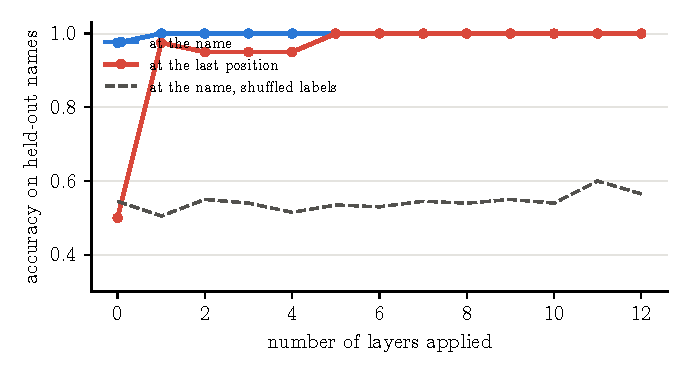
\includegraphics[width=0.58\textwidth]{figures/fig_probe_layers.pdf}
\caption{Accuracy of linear probes for the gender of a name on 40 held-out names (\cref{exp:probe}). The
horizontal axis is the number of layers that have been applied before the stream is read.}
\label{fig:probe}
\end{figure}

\paragraph{From a probe to a direction.} There is a second, simpler way to estimate a direction, and it needs no
training. The \emph{difference of means} is the vector $\E[x\mid y=1]-\E[x\mid y=0]$, which we estimate by the
difference of the two sample averages. If \eqref{eq:lrh} holds with equality, we can say exactly what this vector
measures. By linearity of the expectation,
\begin{equation}\label{eq:diffmeans}
\E[x\mid y=1]-\E[x\mid y=0] \;=\; \sum_{j=1}^{N}\big(\E[f_j\mid y=1]-\E[f_j\mid y=0]\big)\,v_j .
\end{equation}
Suppose that the label indicates the presence of feature $j$, and that every other feature has the same average
in both classes. Then only the term of feature $j$ is nonzero, and the difference of means is a positive multiple of
$v_j$. If some other feature is more frequent in one class than in the other, its direction is mixed into the
difference of means. Equation \eqref{eq:diffmeans} therefore also tells us how to collect data: the two classes
should differ in the concept of interest and in nothing else. Our two sets of prompts satisfy this, because they
differ only in the name.

\subsection{Steering: is the direction used?}

A probe shows that some information is present in an activation. It does not show that the model actually uses
this information. To test whether the model uses it, we have to change the activation along the direction and
observe how the output changes. Let $v\in\R^d$ be a direction and $\eta$ a real number. \emph{Steering}, also
called activation addition, replaces a stream vector $x$ by
\begin{equation}\label{eq:actadd}
x+\eta\,v
\end{equation}
at a chosen layer and position. The rest of the computation then proceeds as usual
\citep{turner2023steering,rimsky2024steering}.

\begin{experiment}[Steering a name from male to female]\label{exp:steer} \script{exp\_directions.py}
Let $v$ be the difference of means between female and male names. We compute it from the 72 training names, at
the input of layer 4 and at the position of the name. The norm of $v$ is $26$, about a third of the norm of a
typical stream vector at this place. We add $\eta v$ to the stream of the 20 held-out \emph{male} names and measure
the logit difference between the two pronouns (\cref{fig:steer}, left). Without steering, the logit difference is
$-3.3$. With $\eta=1$, which moves an average male name to an average female name, it is $+2.4$. This is close to
the value $+2.9$ of the held-out female names. With $\eta=-1$, the prediction becomes even more male, with a logit
difference of $-4.7$. We also add random directions of the same length with the same values of $\eta$. On average
over five random directions, they change the logit difference by at most $0.6$.

So this direction is not only correlated with gender. Moving along it changes the behaviour of the model in the
predicted way, while moving along random directions does not. In this example, this is causal evidence for
\cref{def:lrh}.
\end{experiment}

\begin{figure}[t]
\centering
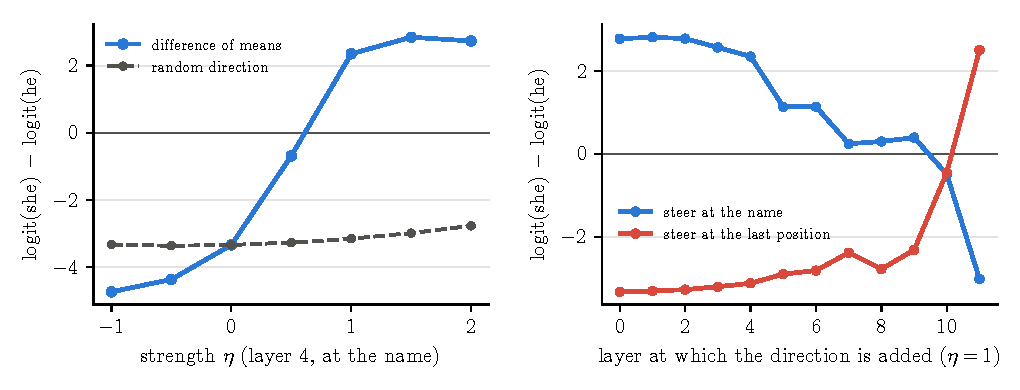
\includegraphics[width=0.95\textwidth]{figures/fig_steering.pdf}
\caption{Steering the gender of a name in GPT-2 small (\cref{exp:steer,exp:decodable}), measured on 20 held-out
male names. Left: adding $\eta$ times the difference of means at the name, at the input of layer 4, compared
with random directions of the same length. Right: adding the difference of means of each layer with $\eta=1$, at
the name and at the last position.}
\label{fig:steer}
\end{figure}

\begin{experiment}[Decodable is not the same as used]\label{exp:decodable} \script{exp\_directions.py}
We now repeat the steering with $\eta=1$ at every layer, once at the position of the name and once at the last
position. Each time we use the difference of means that is computed at that layer and position (\cref{fig:steer},
right).

At the position of the name, steering at the input of layers 0 to 4 changes the logit difference from $-3.3$ to
values between $+2.4$ and $+2.8$. The effect then becomes smaller in steps. The logit difference is $+1.1$ for
steering at layers 5 and 6, between $+0.2$ and $+0.4$ at layers 7 to 9, $-0.5$ at layer 10, and $-3.0$ at layer 11.
The last value is the same as without steering. A change at the input of layer $\ell$ can only affect the heads of
layer $\ell$ and of later layers. So a drop between steering at layer $\ell$ and steering at layer $\ell+1$ shows
that heads of layer $\ell$ read the gender from the position of the name. The curve drops after layers 4, 6 and 9,
and the largest drop is after layer 10. A change at the name after layer 10 comes too late to affect the
prediction.

At the last position, the curve behaves in the opposite way, and the result is surprising. Up to layer 9,
steering changes the logit difference by at most about one logit. Steering at layer 10 moves it to $-0.5$, and only
steering at layer 11 changes the predicted pronoun. But \cref{exp:probe} showed that a probe can read the gender at
the last position with $95\%$ to $100\%$ accuracy from layer 1 onwards. So for nine layers the information is
present at the last position, and a probe can find it, but the prediction of the model hardly depends on it. The
model uses the information at the position of the name instead, and most of this information is moved to the last
position only in layer 10.
\end{experiment}

\begin{caution}
\Cref{exp:decodable} teaches the most important lesson about probes. A probe shows a correlation between an
activation and a label. Whether the model uses the information has to be tested with an intervention. We add two
further warnings. First, a probe with many parameters can learn the task by itself, even if the model has not
computed the property. For this reason, probes are kept linear and are compared with a control task
\citep{hewitt2019designing}. Second, the direction of the probe need not be the direction that the model uses. In
our experiment, the probe direction at layer 4 has a cosine of $0.86$ with the difference of means. Steering along
the probe direction, scaled to the same length, moves the logit difference only to $+1.7$ instead of $+2.4$.
\citet{marks2024geometry} observed the same for directions that encode whether a statement is true.
\end{caution}

\subsection{What has been found this way}

Several of the best-known results of mechanistic interpretability combine the two tools of this session: a
direction is found by observation and then tested by steering. We report three of these results.

\begin{itemize}
\item \textbf{A model of a board game.} \citet{li2023emergent} trained a transformer to predict legal moves in
the board game Othello. The model only saw sequences of moves, never the board. Linear probes for the state of each
square (black, white or empty) had an error of more than $20\%$, while probes with one hidden layer had an error
below $2\%$. Changing the activations according to the probe changed the moves that the model predicted. Later,
\citet{nanda2023emergent} found that a \emph{linear} probe works well if it is trained on a different label: whether
a square holds a piece of the player whose turn it is, or a piece of the opponent. So the information was stored
linearly all along, but in terms of a variable that the first study had not tried.
\item \textbf{Refusal.} Chat models are trained to refuse harmful requests. \citet{arditi2024refusal} computed
the difference of means between the streams on harmful instructions and the streams on harmless instructions. In 13
openly available chat models with up to 72 billion parameters, they found the same two results. When they removed
the component along this direction from the stream at all layers and positions, the model no longer refused
harmful requests. When they added the direction, the model refused harmless requests.
\item \textbf{Not every concept is a single direction.} \citet{engels2025not} found that GPT-2 and Mistral 7B
represent the days of the week and the months of the year as points on a circle in a two-dimensional subspace. So
\cref{def:lrh} is a useful first approximation, but it has exceptions.
\end{itemize}

\begin{takeaways}
The main working hypothesis of mechanistic interpretability is that a model represents concepts as directions in
the space of its activations. A linear probe tests whether a concept can be read linearly from an activation, and
the difference of means estimates a direction without training. Only an intervention shows whether the model uses
a direction. In GPT-2 small, a probe can read the gender of a name almost everywhere. Steering shows that the model
reads the gender from the position of the name, mostly as late as layer 10, and that the copy at the last position
matters only at the very end.
\end{takeaways}

\subsection*{Questions for the seminar}

\begin{exercise}[A contaminated direction]\label{ex:contaminated}
Let $x=f_1v_1+f_2v_2$ with orthonormal vectors $v_1,v_2$ and $f_1,f_2\in\{0,1\}$. The label is $y=f_1$. In the data
set, feature $2$ is present in $80\%$ of the examples with $y=1$ and in $20\%$ of the examples with $y=0$.
(a) Compute the difference of means with \eqref{eq:diffmeans}. (b) Compute the cosine of the angle between it
and $v_1$. (c) We steer with this vector in order to switch on the first concept. What else happens? (d) How
should the data set be changed?
\end{exercise}

\begin{exercise}[The probe direction is not the difference of means]\label{ex:lda}
Suppose that $x$ is Gaussian with mean $\mu_1\in\R^d$ if $y=1$ and Gaussian with mean $\mu_0\in\R^d$ if $y=0$, in
both cases with the same invertible covariance matrix $\Gamma$, and that both classes are equally likely.
(a) Show that the logarithm of $\Pr(y=1\mid x)/\Pr(y=0\mid x)$ equals $w^\top x+b_{\mathrm{probe}}$ with
$w=\Gamma^{-1}(\mu_1-\mu_0)$ and a suitable number $b_{\mathrm{probe}}$, so that the probe \eqref{eq:probe} with this
$w$ is exactly right. (b) Let $d=2$, $\mu_1-\mu_0=(1,0)^\top$ and
$\Gamma=\begin{pmatrix}1&\rho\\ \rho&1\end{pmatrix}$ with $0<\rho<1$. Compute $w$ up to a positive factor. (c) The
classes differ only in the first coordinate. Why does the probe still use the second
coordinate? (d) Relate this to
the numbers $0.86$, $+1.7$ and $+2.4$ of the Caution box.
\end{exercise}

\begin{exercise}[Reading the two curves]\label{ex:curves}
In the right panel of \cref{fig:steer}, the two curves cross at layer 10. (a) Which kind of component must be
responsible for the fact that the gender of the name reaches the last position at all? (b) Steering at the
input of layer 10 gives about $-0.5$ at both positions. Steering at the input of layer 11 gives $-3.0$ at the
name and $+2.5$ at the last position. Explain how these four numbers fit together. (c) Design an experiment with
the tools of session 2 that would find the components of (a).
\end{exercise}

\begin{exercise}[What a failed probe shows]\label{ex:othello}
In the Othello study, a probe with one hidden layer decoded the colour of each square and a linear probe did
not. (a) State two different hypotheses about the model that are both consistent with this pair of results.
(b) Which of them is supported by the later finding about ``my piece or the opponent's piece''? (c) What does
the episode teach about negative probing results?
\end{exercise}

\begin{readinglist}
\item \citet{park2024linear}, \emph{ICML}. Makes the linear representation hypothesis precise and separates
several meanings of ``linear''.
\item \citet{hewitt2019designing}, \emph{EMNLP}. Control tasks for probes, the standard guard against a probe that
does the work itself.
\item \citet{li2023emergent}, \emph{ICLR}. The Othello study. The paper is short, and it is a good example of a probing study that tests its probe
with an intervention.
\item \citet{arditi2024refusal}, \emph{NeurIPS}. The refusal direction. The clearest example of a behaviour of
large models that is controlled by one direction.
\item \citet{marks2024geometry}, \emph{COLM}. Directions for the truth of a statement, with a careful comparison of
the difference of means and logistic regression.
\end{readinglist}
